%
In this section we will describe the user interface design of the system. We will provide a mockup of the main pages of the system and a description of the main functionalities of the system.

The user interface of the system is designed to be simple and intuitive. As the system is intended to be used with a desktop browser, the interfaces presented here are based on a desktop browser, but the interface is thought to be responsive and consequently usable also on mobile devices.

\section*{Common Interfaces}
\label{s:common_interface}%
Some pages of the platform are common, or very similar, for both ST and ED, so in this section we will show only once the mockup of the pages and we will describe the functionalities of the pages for both ST and ED.

\subsubsection*{Login Page}
\label{ss:login}%

\begin{figure}[H]
  \centering
  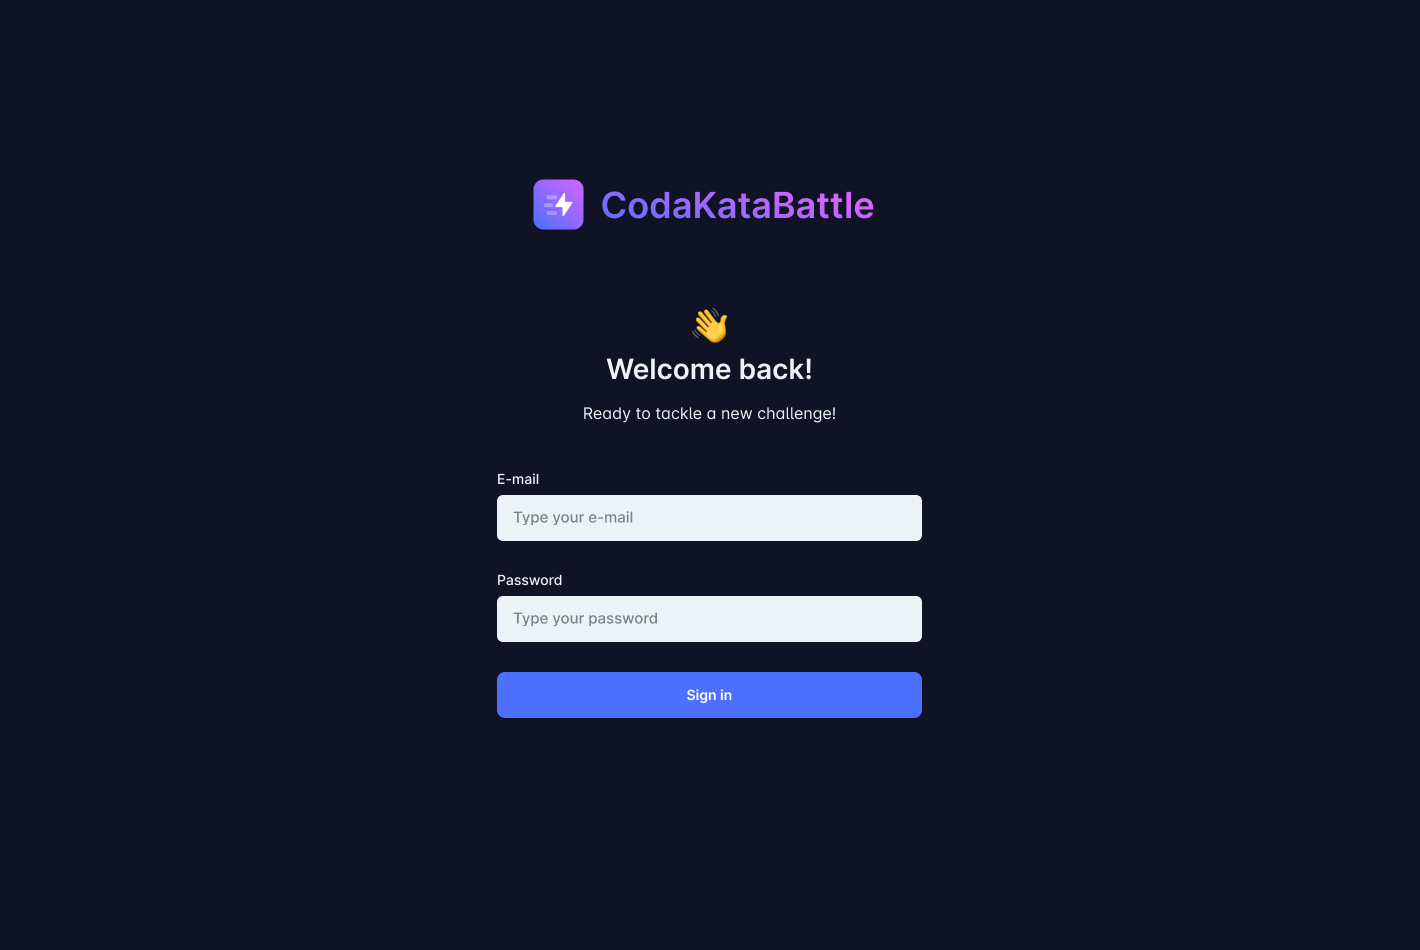
\includegraphics[width=\textwidth]{User Interface/Login.png}
  \caption{CKB login page}
  \label{fig:login}
\end{figure}

\newpage

\subsubsection*{Registration Page}
\label{ss:registration}%
Here for simplicity we show only the registration page for a ST, but the registration page for a ED is equal to this one with the only difference that the ED is required to insert also information about the institution he/she works for.

\begin{figure}[H]
  \centering
  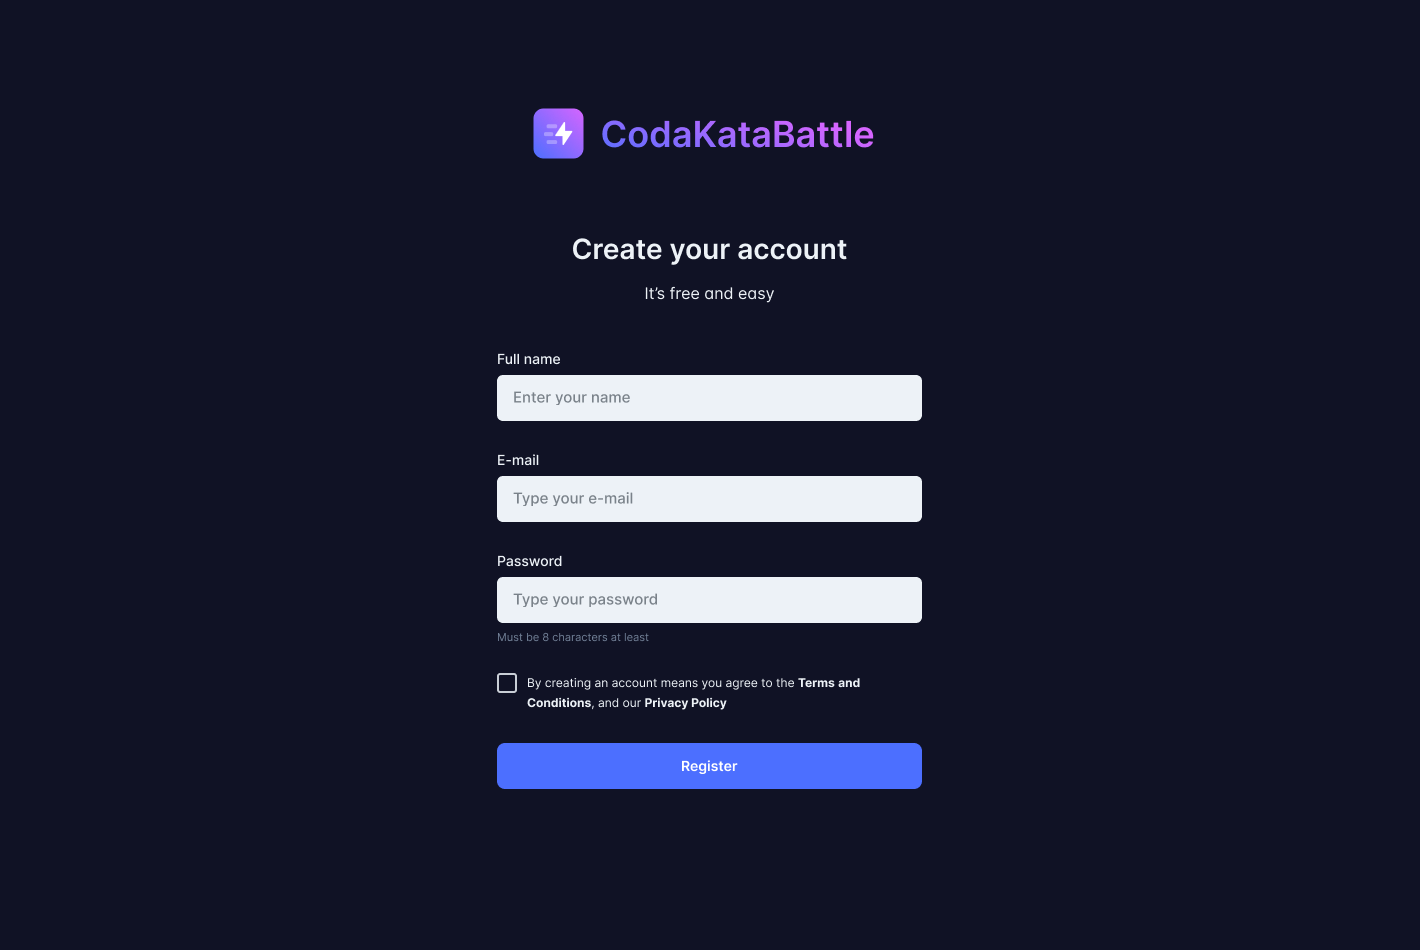
\includegraphics[width=\textwidth]{User Interface/Register.png}
  \caption{CKB registration page}
  \label{fig:registration}
\end{figure}

\newpage

\subsubsection*{Home Page}
\label{ss:home_page}%
This is a mockup of the homepage of a ST. ED would see a very similar home page with statistics about the competition and battle created.

\begin{figure}[H]
  \centering
  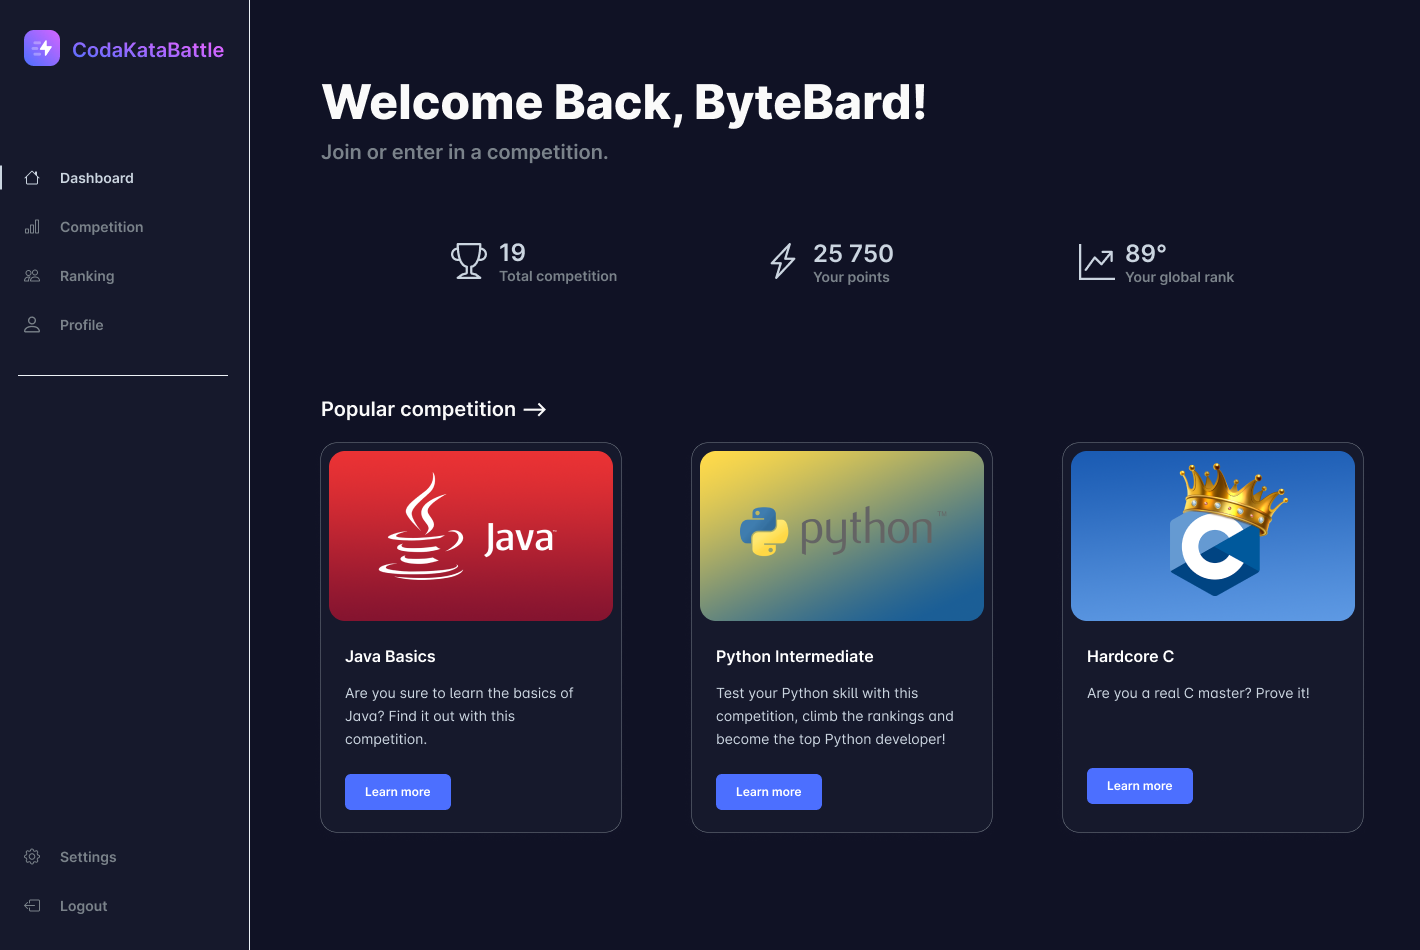
\includegraphics[width=\textwidth]{User Interface/Homepage Student.png}
  \caption{CKB student home page}
  \label{fig:homepage}
\end{figure}

\newpage

\subsubsection*{Competition Page}
\label{ss:competition_page}%
In this page the ST can see the list of all the competitions he/her is currently enrolled in. The ED can see the list of all the competitions he/her has created.

\begin{figure}[H]
  \centering
  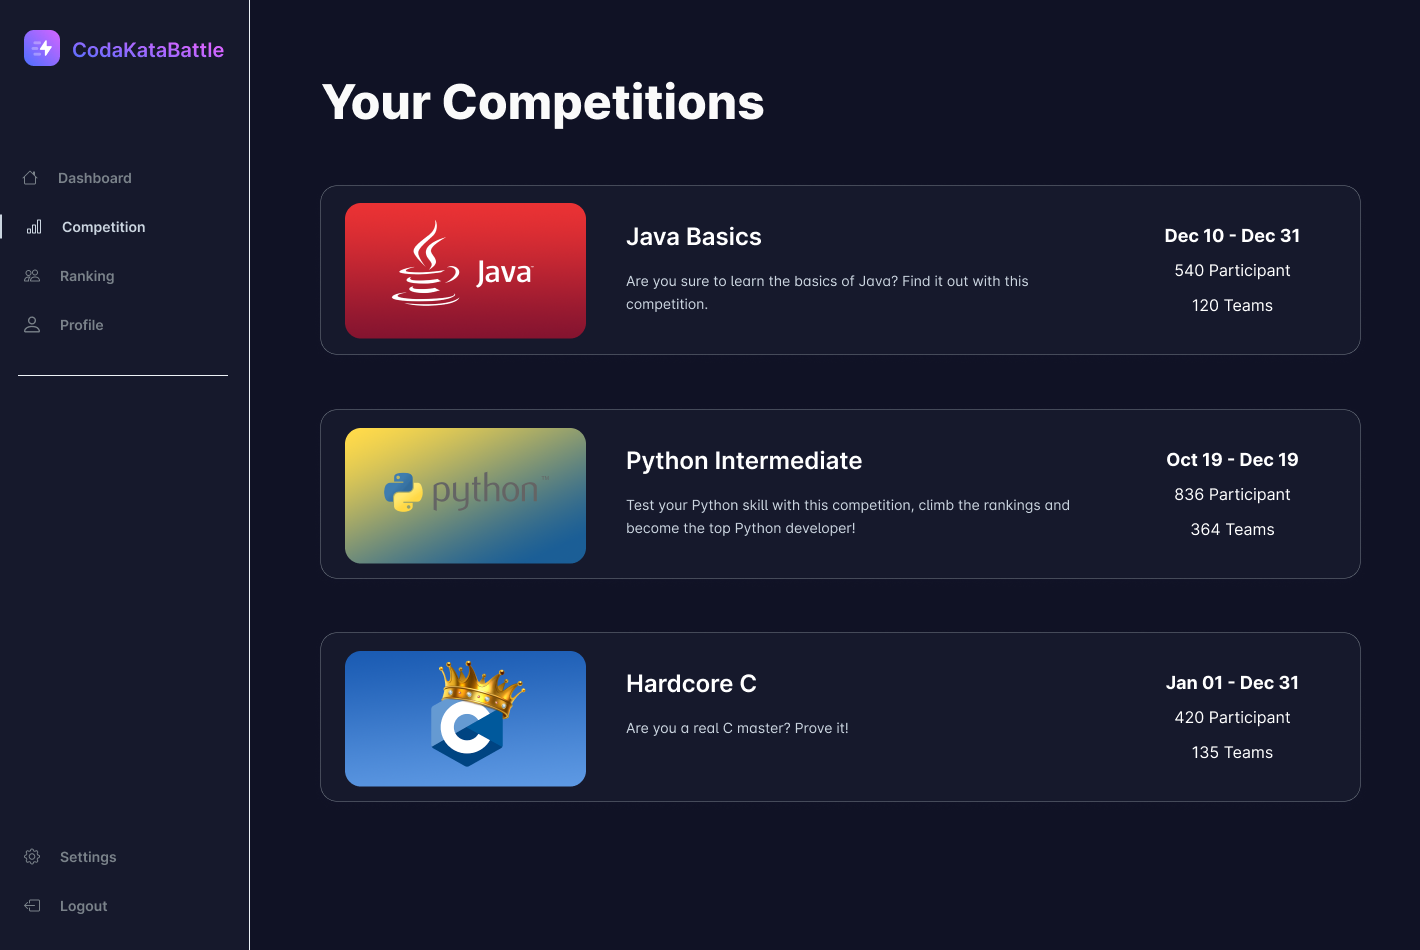
\includegraphics[width=\textwidth]{User Interface/Competition.png}
  \caption{CKB competition page}
  \label{fig:competition}
\end{figure}

\newpage

\subsubsection*{Ranking Page}
\label{ss:ranking_page}%
This is a the mockup of all the rankings present in the system. In particular, this is equal for the global ranking, competition raning and battle ranking pages. Both the ST and the ED are presented with the same interface and functionalities when consulting the ranking pages.

\begin{figure}[H]
  \centering
  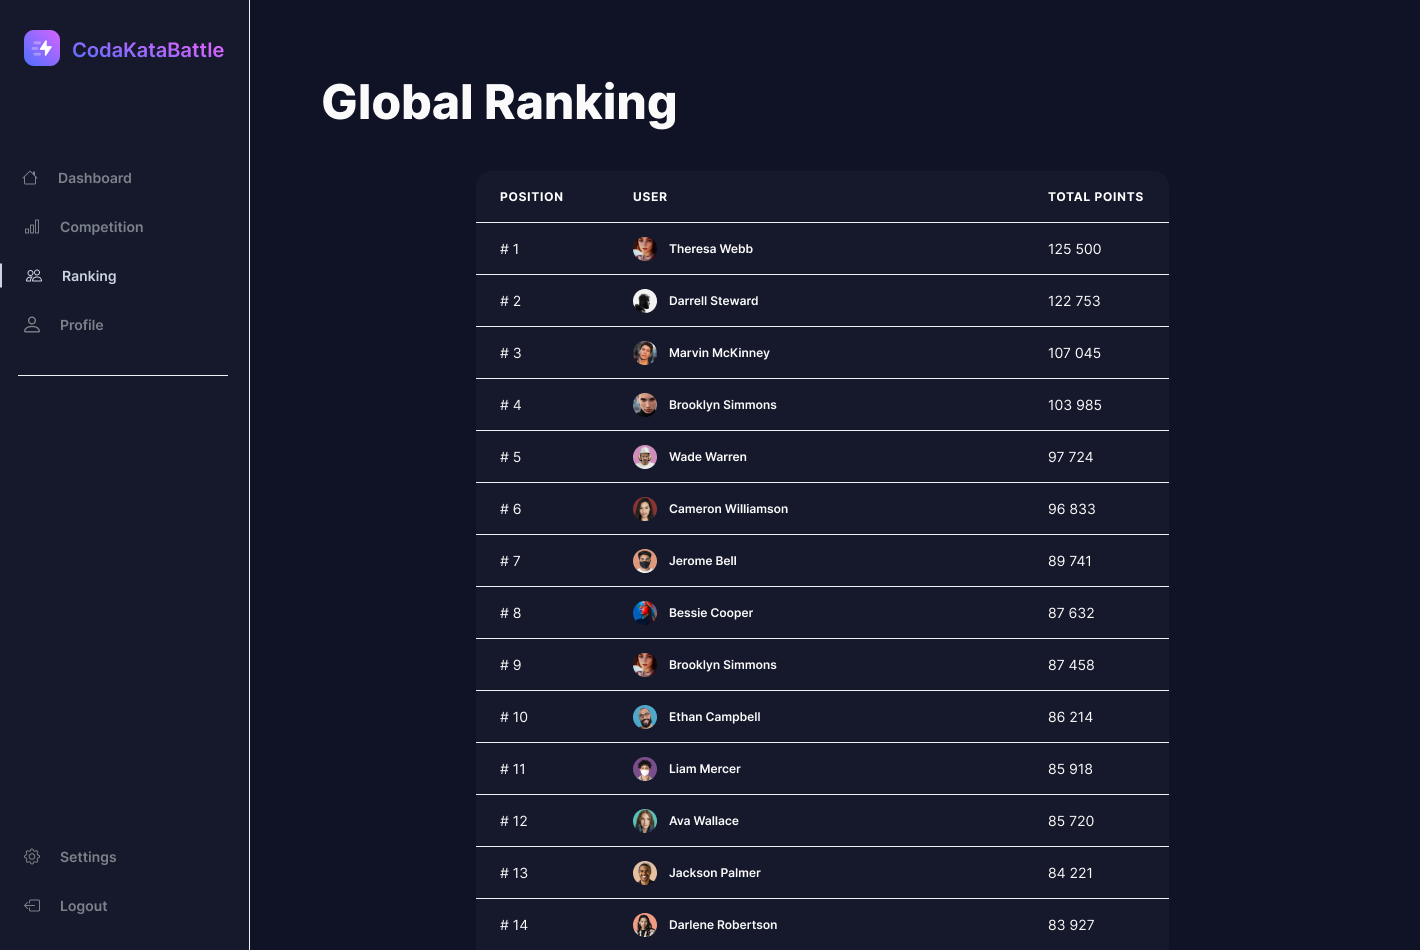
\includegraphics[width=\textwidth]{User Interface/Ranking.png}
  \caption{CKB global ranking page}
  \label{fig:ranking}
\end{figure}

\newpage

\subsubsection*{ST Profile Page}
\label{ss:ST_profile_page}%
Also this page is equal for both ST and ED. In particular in this page it is possible to see all the badges earned by the ST, other than the information about the competition he/her has partecipated in and their statistics.

\begin{figure}[H]
  \centering
  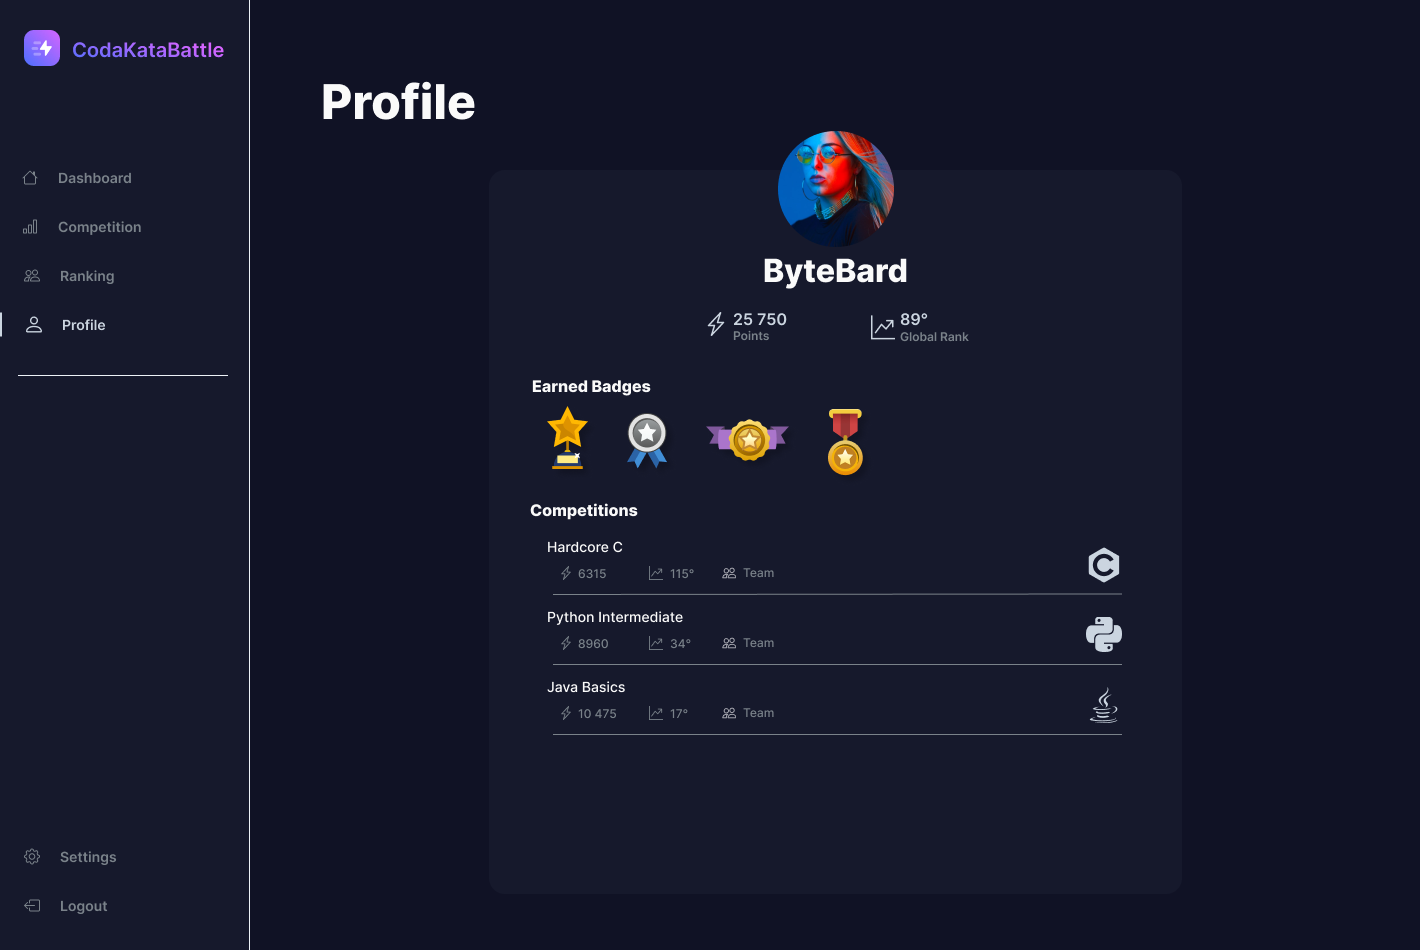
\includegraphics[width=\textwidth]{User Interface/Profile Student.png}
  \caption{CKB ST profile page}
  \label{fig:ST_profile}
\end{figure}

\newpage

\section*{ST Interfaces}
\label{s:ST_interface}%

Now are presented the interfaces that are specific for the ST, in particular are shown the pages relative to the join of a battle by the ST.

\subsubsection*{Join Battle Pages}
\label{ss:join_battle_pages}%
To create a more pleasant experience for the ST, the join battle pages are divided in different steps. In particular, the first step is to choose to join with a T or as a single ST. In the second step, if the ST has decided to join as a T he/her has to choose if he/her wants to create a new T or join an existing one. In case the ST has decided to create a new T is presented with the relative page, otherwise he/her is presented with the page to join an existing public T.

\begin{figure}[H]
  \centering
  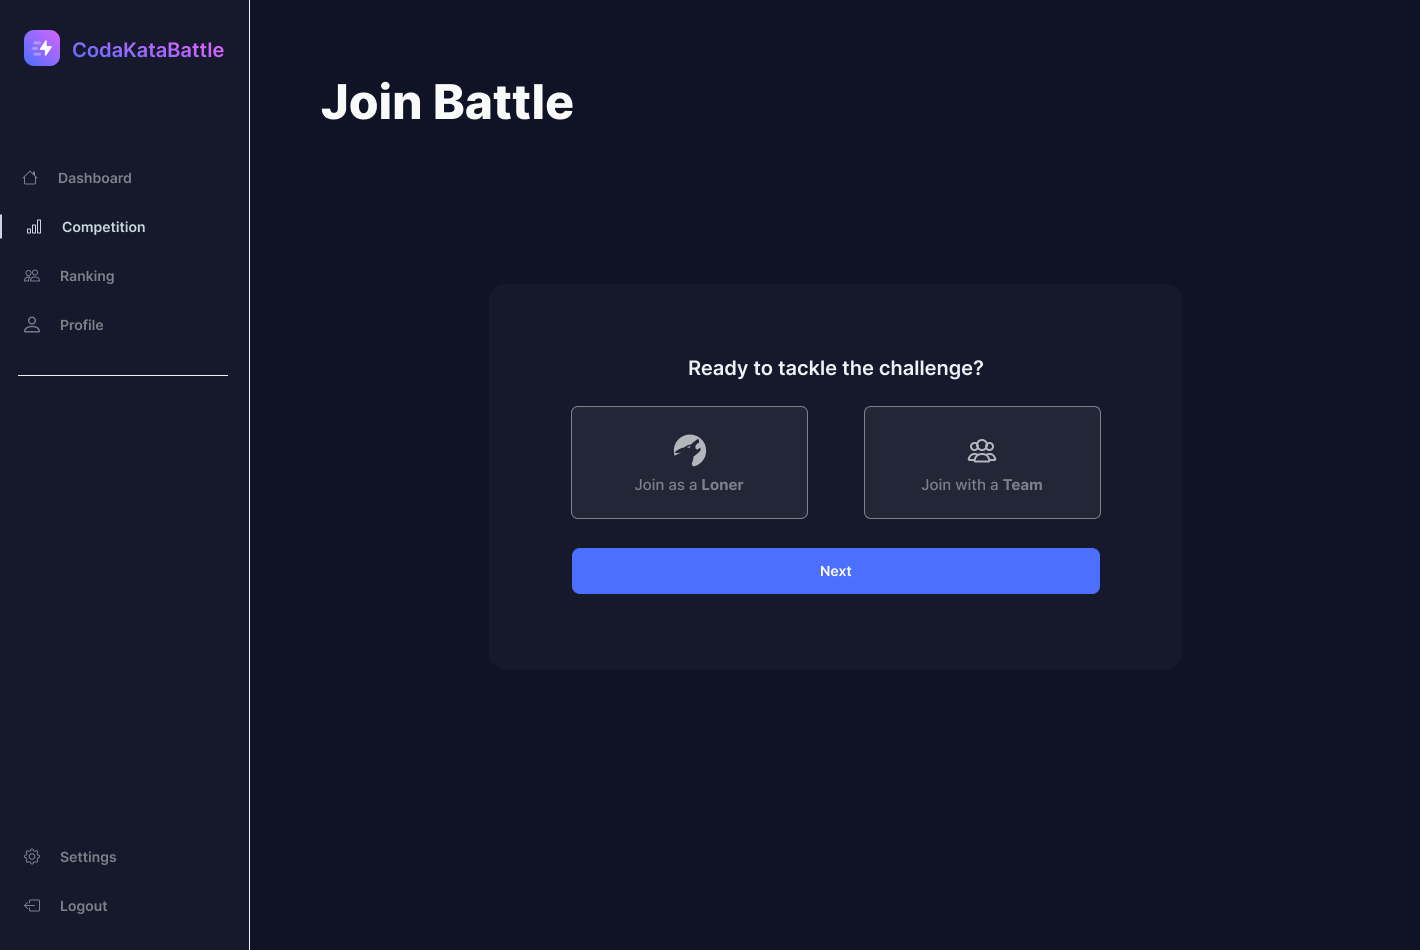
\includegraphics[width=\textwidth]{User Interface/Join Battle Student - 1.png}
  \caption{Join battle page - step 1}
  \label{fig:join_battle1}
\end{figure}

\begin{figure}[H]
  \centering
  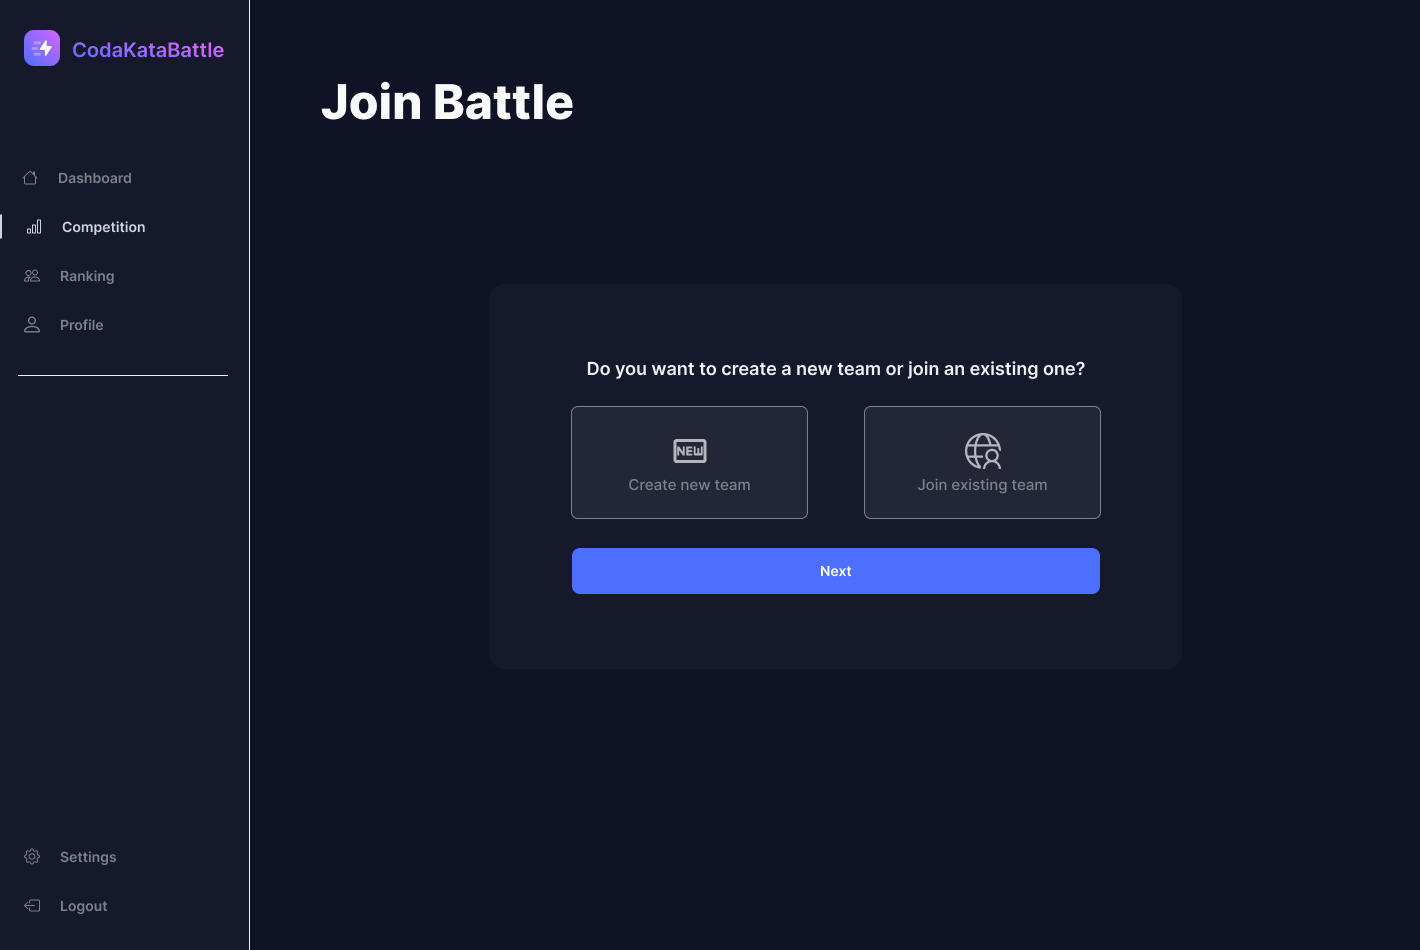
\includegraphics[width=0.95\textwidth]{User Interface/Join Battle Student - 2.png}
  \caption{Join battle page - step 2}
  \label{fig:join_battle2}
\end{figure}

\begin{figure}[H]
  \centering
  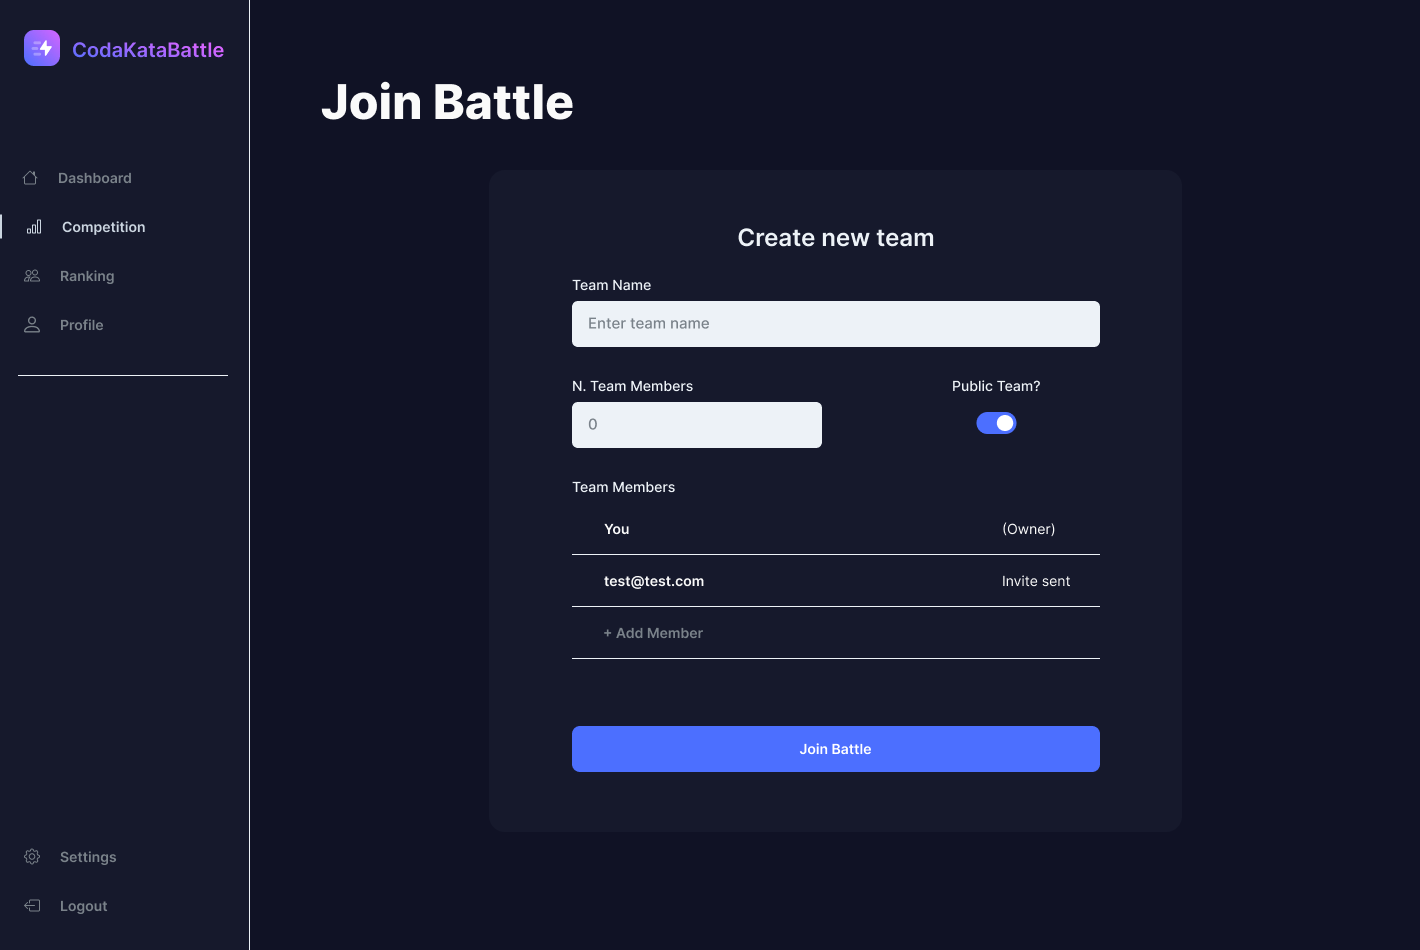
\includegraphics[width=0.95\textwidth]{User Interface/Join Battle Student - 3.png}
  \caption{Create a new team}
  \label{fig:join_battle3}
\end{figure}

\begin{figure}[H]
  \centering
  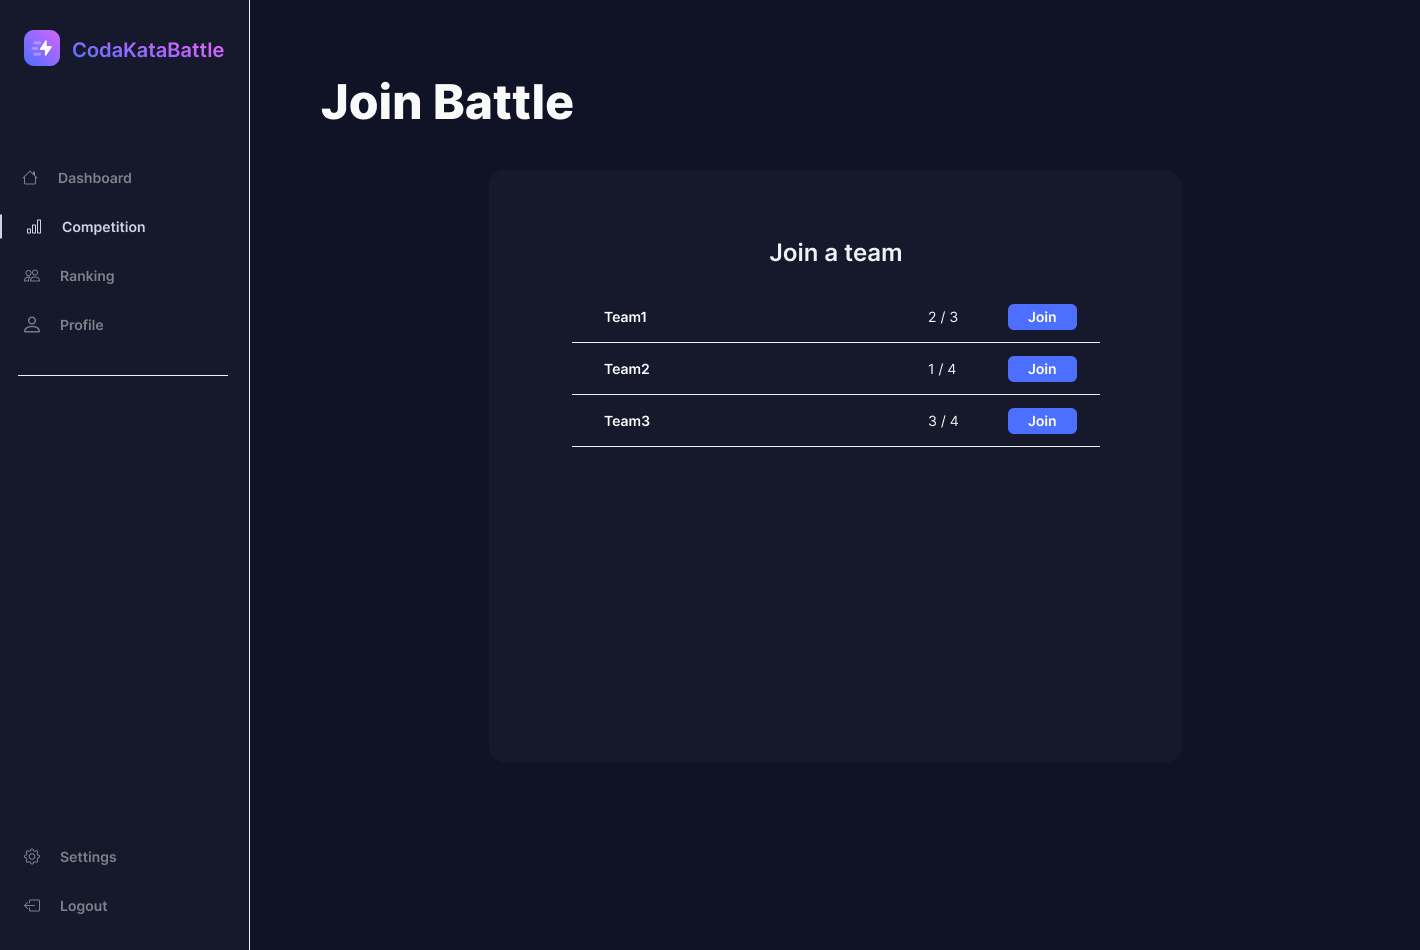
\includegraphics[width=\textwidth]{User Interface/Join Battle Student - 4.png}
  \caption{Join a public team}
  \label{fig:join_battle4}
\end{figure}

\newpage

\section*{ED Interfaces}
\label{s:ED_interface}%

In this section are presented the interfaces that are specific for the ED, in particular are shown the pages relative to the creation of a competition, the creation of a battle and the creation of a badge.

\subsubsection*{Create Competition Page}
\label{ss:create_competition_page}%

\begin{figure}[H]
  \centering
  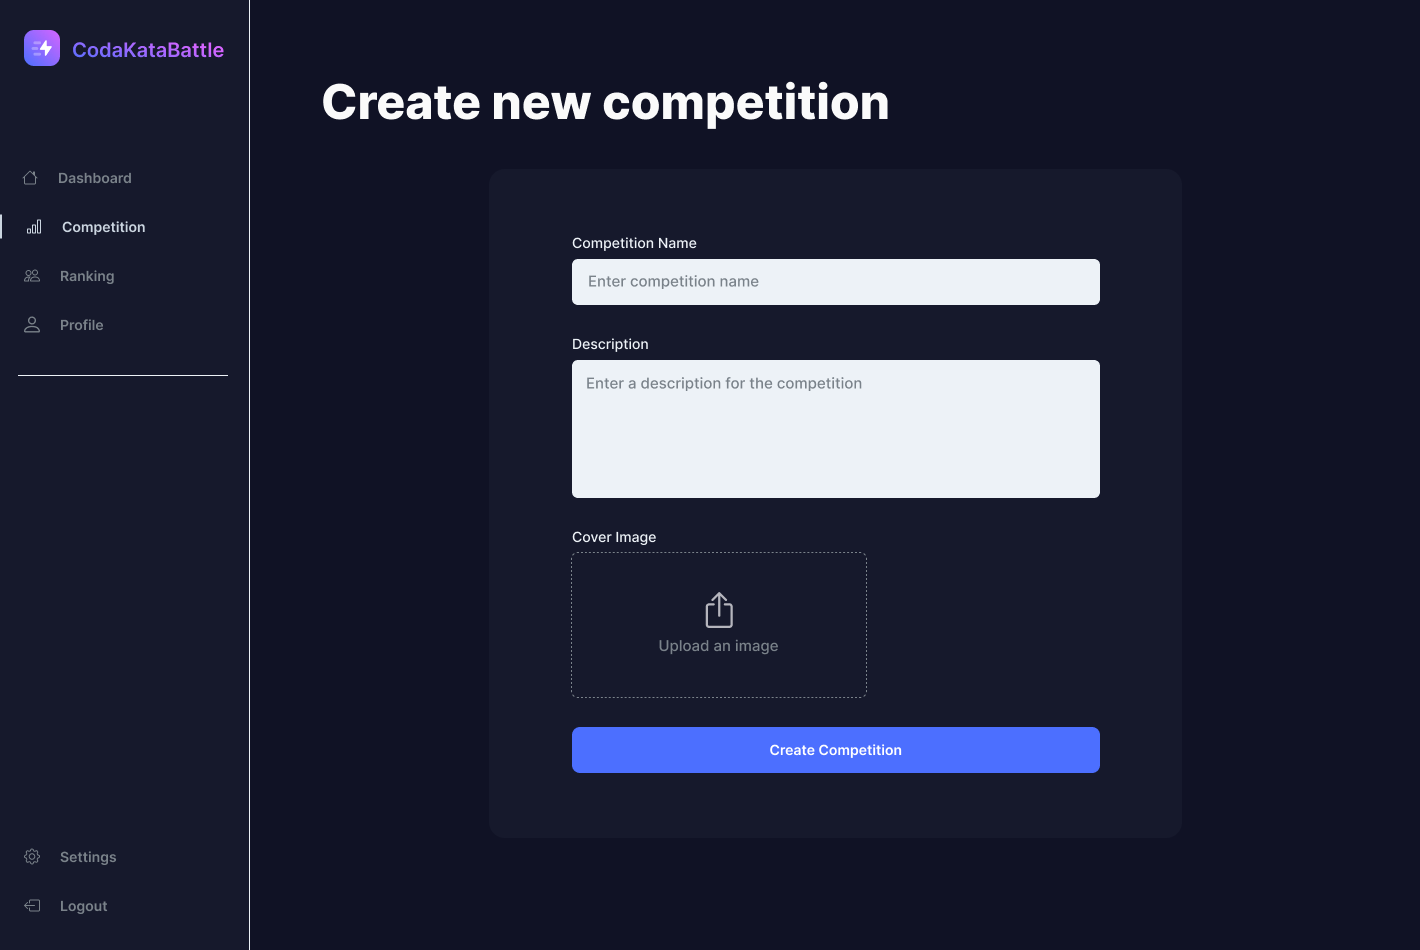
\includegraphics[width=\textwidth]{User Interface/Create Competition Educator.png}
  \caption{CKB create competition page}
  \label{fig:create_competition}
\end{figure}


\subsubsection*{Create Battle Pages}
\label{ss:create_battle_pages}%
As for the join of a battle for a ST also the creation of a battle is divided in two different steps. In the first step the ED has to insert all the general information about the battle, while in the second step he/her has to insert the code and settings for the automatic evaluation of the code.

\begin{figure}[H]
  \centering
  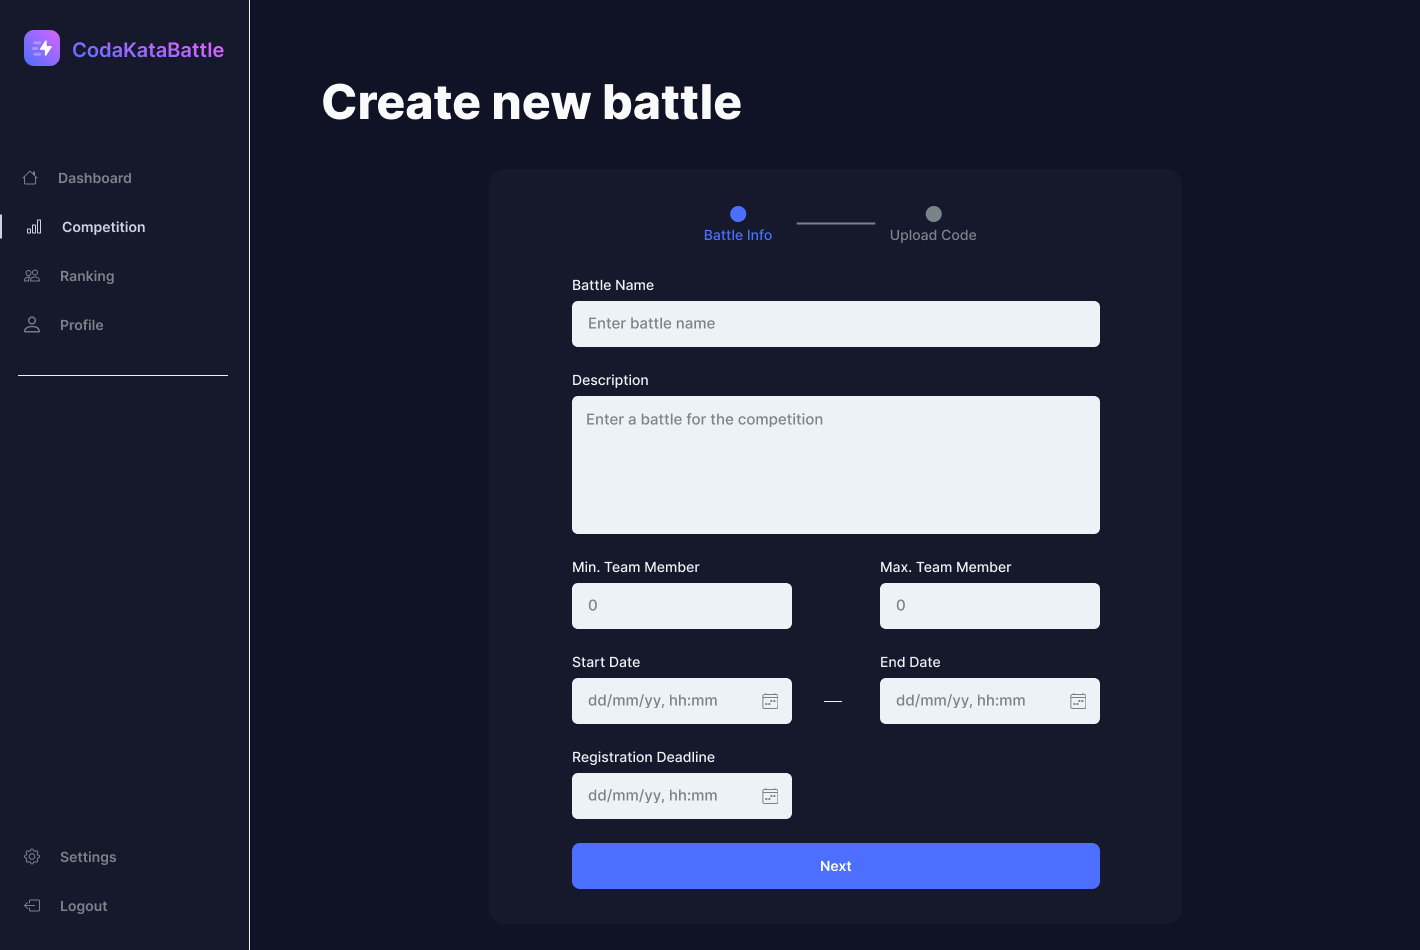
\includegraphics[width=0.95\textwidth]{User Interface/Create Battle Educator - 1.png}
  \caption{CKB create battle page - step 1}
  \label{fig:create_battle1}
\end{figure}

\begin{figure}[H]
  \centering
  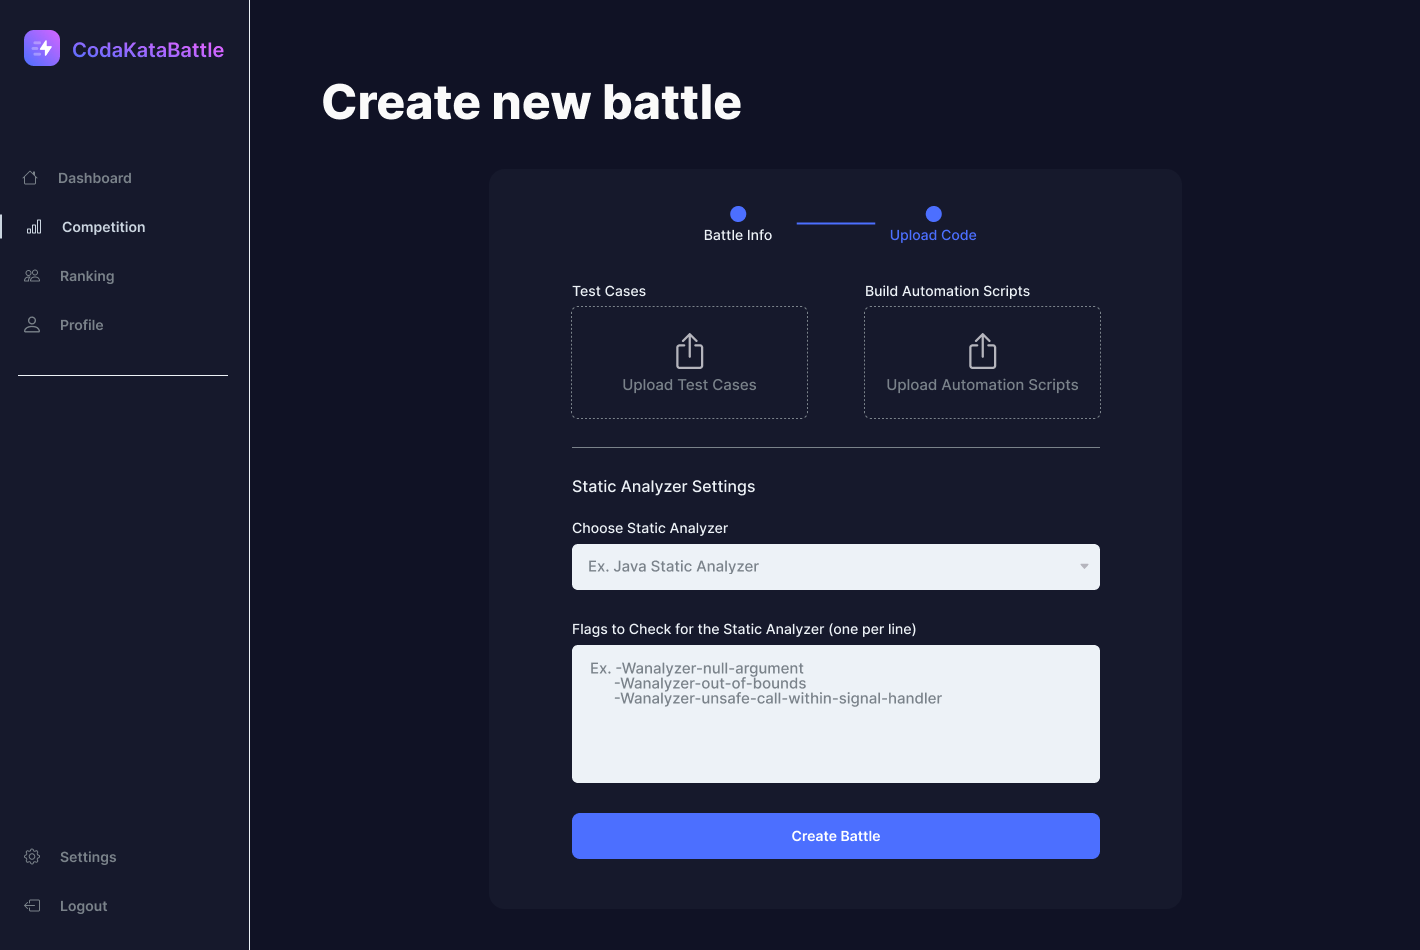
\includegraphics[width=0.95\textwidth]{User Interface/Create Battle Educator - 2.png}
  \caption{CKB create battle page - step 2}
  \label{fig:create_battle2}
\end{figure}


\subsubsection*{Create Badge Pages}
\label{ss:create_badge_pages}%
Similarly to the last function, the creation of a badge is divided in two steps. In the first step the ED can insert all the information of the badge, that include the name of the badge, a description and a picture. In the second step the ED can choose the criteria that the ST has to satisfy to earn the badge, this is done by a set of pre-defined criteria that the ED can choose from.

\begin{figure}[H]
  \centering
  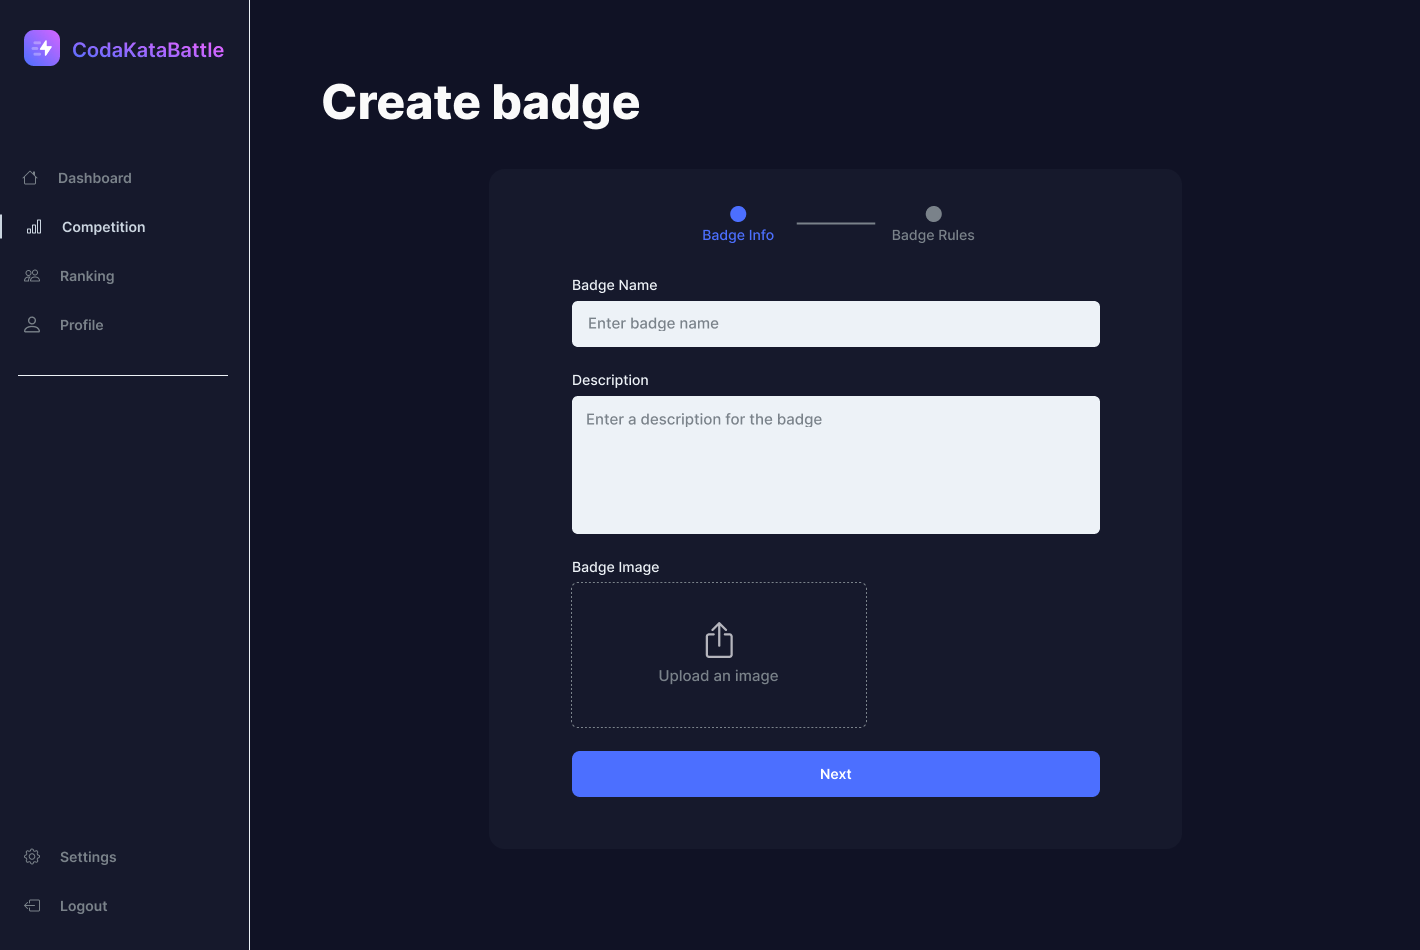
\includegraphics[width=\textwidth]{User Interface/Create Badge Educator - 1.png}
  \caption{CKB create badge page - step 1}
  \label{fig:create_badge1}
\end{figure}

\begin{figure}[H]
  \centering
  \includegraphics[width=\textwidth]{User Interface/Create badge Educator - 2.png}
  \caption{CKB create badge page - step 2}
  \label{fig:create_badge2}
\end{figure}

\newpage

\subsubsection*{Manual Evaluation Page}
\label{ss:manual_evaluation_page}%
This is the page where the ED can manually evaluate the code of a T. In particular, the ED can see some information about the latest submission of a T and can visit GitHub to see the code of the T. Then the ED can evaluate the latest submission of the T, assigning a score.

\begin{figure}[H]
  \centering
  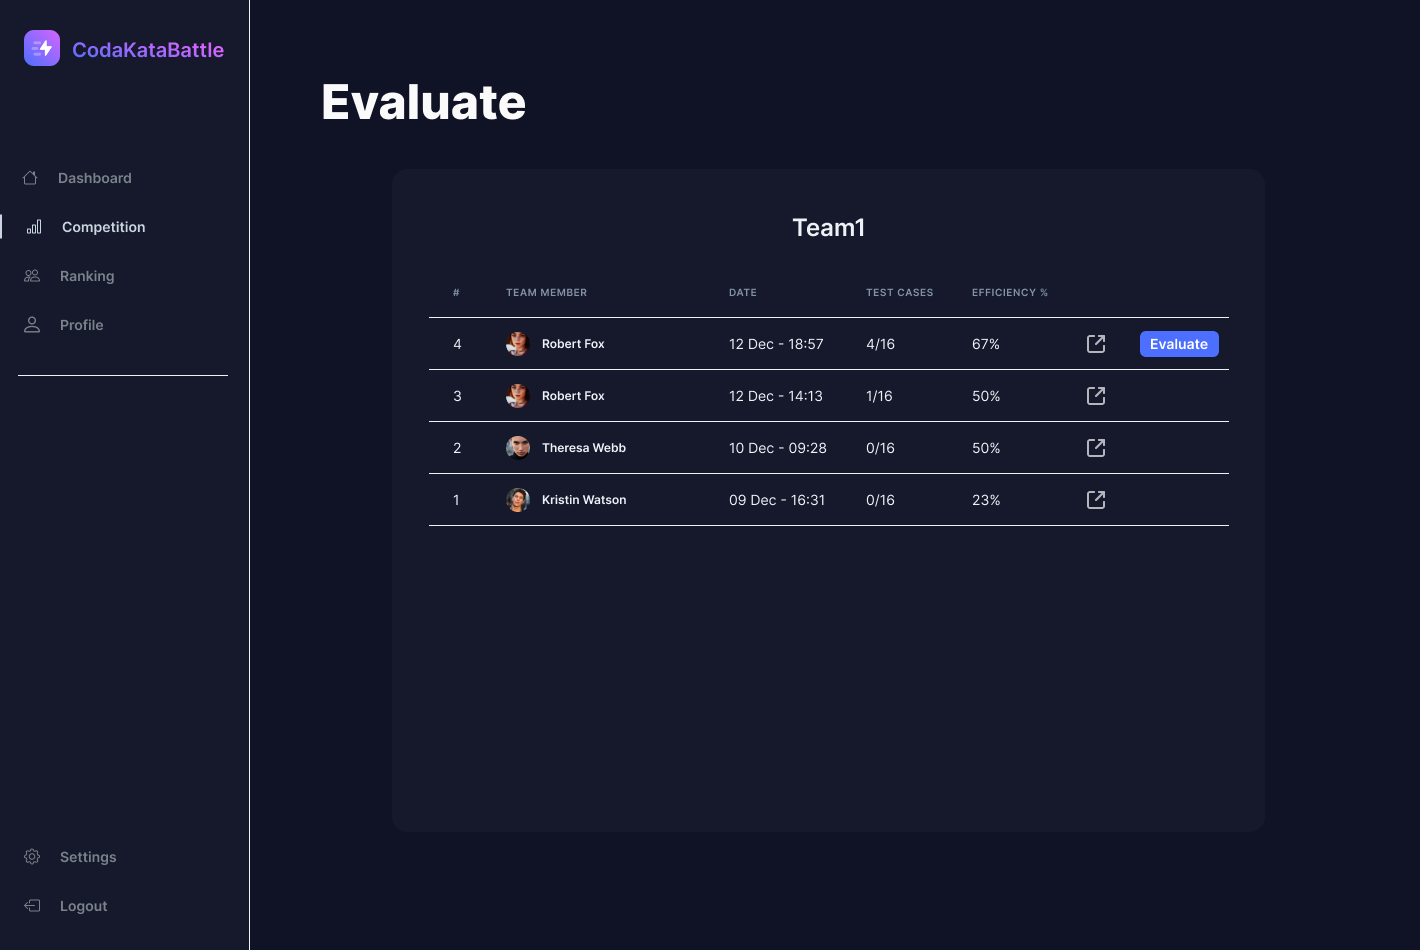
\includegraphics[width=\textwidth]{User Interface/Manual Evaluation Educator.png}
  \caption{CKB manual evaluation page}
  \label{fig:manual_evaluation}
\end{figure}
